\newcommand{\tinymatrix}[1]{ \big(\begin{smallmatrix} #1 \end{smallmatrix}\big) }
\newcommand{\minimatrix}[1]{{\scriptsize\arraycolsep=0.3\arraycolsep\ensuremath{\begin{pmatrix}#1\end{pmatrix}}}}

\chapter{Theory}\label{chapter:theory}

%So what even do I need to talk about here?
%
%Final goal = Higgs (final final goal should actually probably be di-higgs and a discussion of the relevence of this...)
%    What: What is the Higgs?
%    Why: Why do we care about it? It gives things mass and messes with the electroweak interaction
%    When: In what contexts does the Higgs become relevant? The mass of (most) elementary particles and the weak force being weak
%    Where: Where does the higgs fit into the SM? The "Higgs Mechanism"
%    How: How does the higgs mechanism work?

\section{Introduction}

    The Higgs Boson sits as the crown jewel of a grand overarching theory of the behaviour of the universe,
        known as the Standard Model of Particle Physics.
    While its recent discovery has shed light on many of its key properties,
        there are still many details of its nature that are as yet uncomfirmed.
    In this chapter, I want to explain what these properties are and how they can be further studied.
    Moreover, I want to justify why the Higgs is so important as to be worth studying in the first place.
    And to understand the importance of the Higgs Boson, one must understand the structure of the Standard Model itself.

    The structure of the following sections will begin with a discussion of the purpose and fundamental structure of the Standard Model.
    I will follow this with an introduction to the mathematical formalism the Standard Model is based around,
        involving Group Theory, the calculus of variations, and symmetry.
    Here I will introduce the reason for the original postulation of the Higgs, what it is, how it works, and how it fits into the Standard Model.
    Finally, I will motivate further study into the Higgs and provide a technique to perform this study.


%Matter and Forces
%I need to discuss the elementary particles and their organization before I can really discuss the gauge fields.
%Might as well do it here first and foremost
\section{The Standard Model of Particle Physics}
    
    At its core, the Standard Model of Particle Physics is a description of the behaviour and interaction of matter.
    First and foremost then, I want to discuss what this matter actually is.
    All matter can be described as a specific type of elementary particle called a fermion,
        defined by the fact that it contains no discernable substructure and possesses an intrinsic spin of 1/2.
    These particles all have different masses, and are able to interact with each other through three ``fundamental interactions''.
    The three fundamental interactions (more commonly called ``Fundamental Forces'') are known as
        the Electromagnetic, Weak, and Strong interactions (gravity is entirely absent in the Standard Model).
    All the interactions have an associated ``charge'' which can be ascribed to different particles,
        and which govern how strongly that particle can interact with similarly charged particles.
    The various fermions are distinct largely because of the charges they carry.

    \begin{figure}[h!]
        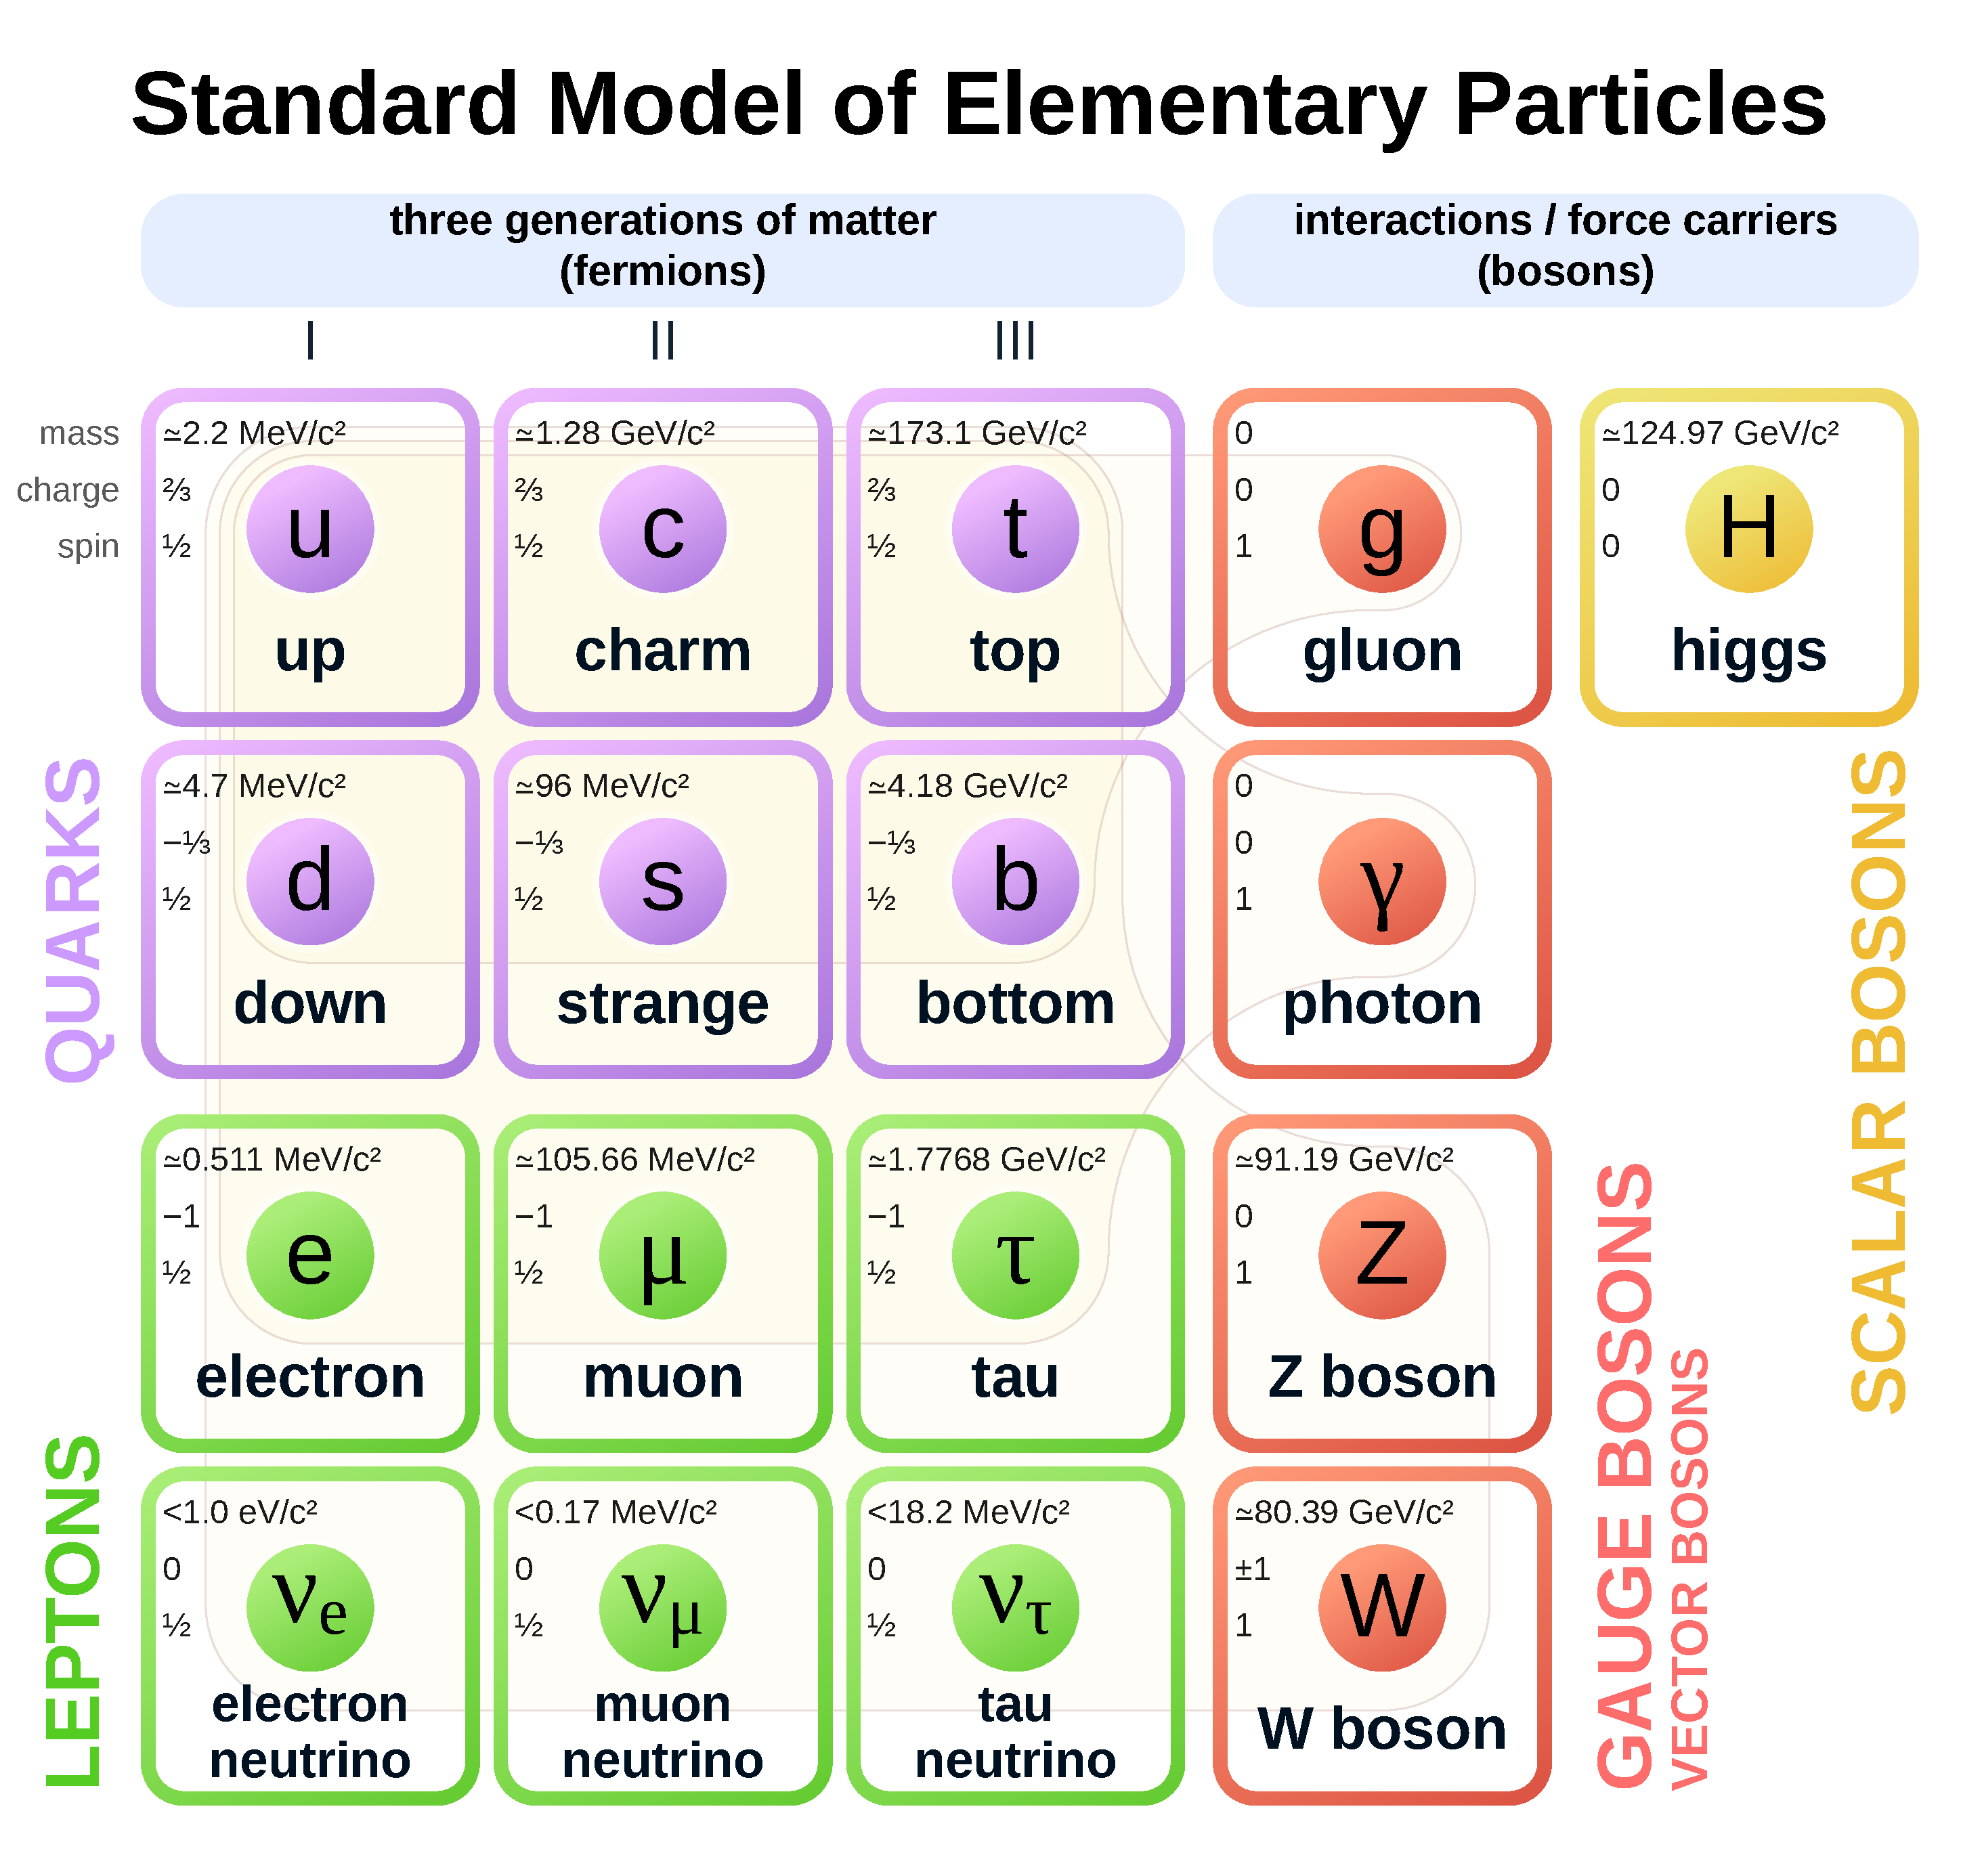
\includegraphics[width=\linewidth,height=\textheight,keepaspectratio]{theory/Standard_Model_of_Elementary_Particles}
        \caption{I'm probably going to need to find something else since this came from wikipedia. I just wanted a placeholder}
        \label{fig:sm_particles}
    \end{figure}
        

    There are twelve distinct elementary fermions (see Figure \ref{fig:sm_particles}),
        which are split evenly into two subgroups, called quarks and leptons.
    Quarks have a charge of 1 with the Strong interaction,
        while leptons have a charge of 0 (and thus cannot interact via the Strong Interaction at all).
    Both classes of particles, quarks and leptons, are divided into three ``generations'' of progressively heavier particles.
    Each generation thus consists of two quarks and two leptons.
    These pairs, called ``doublets'', behave the same across all generations.
    Among the quarks, every generation contains a doublet of an up-type quark (Up, Charm, Top) with electromagnetic charge of 2/3,
        and a down-type quark (Down, Strange, Bottom) with EM charge of -1/3.
    For leptons, each doublet consists of a particle with EM charge of -1, and a neutrino with EM charge of 0.

    In addition to the fermions, there is also an entirely seperate class of particles, called gauge bosons,
        which play a fundamental role in the aforementioned interactions.
    However, the nature of these particles will be discussed later.
    Now, with the enumeration of the various particles complete, it is time to begin the discussion of the Standard Model itself,
        which will serve to explain how these fermions interact with each other.



\section{Composition of Matter: Fields and Dirac Spinors}

    %Fields are a thing.
    The description of matter is governed by the formalism of Quantum Field Theory, which describes particles as pertubations of an overall particle \textit{field}.
    %They're kinda like quantum waves, but not.
    A particle field $\varphi$, describes every particle of the same type at once,
        and particle states $\ket{\varphi}$ correspond to the number of that kind of particle that exists at a given moment.
    The equation of motion used to describe a field varies depending on the properties of the field.
    For a scalar (spinless) field, \phi, the equation of motion is the Klein-Gordon Equation
    \begin{equation} \begin{split}
        p^2 \phi = m^2 \phi
        \\(p^2 - m^2) \phi = 0
    \end{split} \end{equation}
    Recalling the covariant, natural units, quantum mechanical definition of momentum as $p^u = i\partial^u$,
        this can also be written as
    \begin{equation} \begin{split}
        (p^2 - m^2) \phi = 0 \rightarrow (\partial^\mu \partial_\mu + m^2) \phi = 0
    \end{split} \end{equation}

    The Klein-Gordan Equation will be used later when describing the Higgs Field,
        but for now the more important equation is that used for fermions, $\psi$,
        called the Dirac Equation
    \begin{equation}
        (\gamma^\mu p_\mu - m) \psi = 0
        (i\gamma^\mu \partial_\mu  - m) \psi = 0
    \end{equation}

    The Dirac Equation seeks to make the equation of motion first order (i.e.\ only one derivative),
        as this permits a representation of a spinor field.
    Doing this comes with a cost however, as momentum $p_\mu$ is a four-vector, but mass is a scalar.
    The resolution to this problem is a set of four, 4x4 matrices, $\gamma^\mu$, called the gamma matrices.


    %Fields don't describe a single particle, but all particles of the same type at once.
    %Field states are just a count of how many of that particles exist at a given time.
    %Scalar particles are described by Klein Gordon Equation.
    %Spin 1/2 particles are described by dirac equation.
    %It's first order in p, but this requires the gamma matrices.
    %Matrices take many forms, but one of the most revealing is the Weyl, or Chiral, form.
    %Do some math to show fields in chiral form, to show Chirality.


    %It takes from quantum mechanics the uncertainty principle, and from relativity the mass/energy equivalence 
    %It takes from quantum mechanics the wave-like description of position and momentum, along with the uncertainty principle.
    %From special relativity it incorporates the equivalence of space and time, the constance of the speed of light,
    %    and the exchange between mass and energy.
    %Combining the energy/time uncertainty principle with mass/energy equivalence in particular
    %    has the outcome that the number of particles for a given system need not remain constant.
    %To account for this, particles are not described as waves as with the Schrodinger Equation, but rather as ``fields''.
    %A fermion field, $\psi$, does not describe a single particle, but rather all possible fermion for the same kind of particle.
    %For instance, there is a seperate fermion field to describe electrons, up-quarks, and so forth.

    
    describe gamma matrices

    describe anti particle psi bar

    describe chiral representation
    

    %What is the Universe made of (If you stick to this format at all, keep this section brief):

    %%Position and Momentum: Quantum Mechanics
    %   The position and momentum of that matter:
    %       Described via the Canonical Commutation Relation and the formalism of Quantum Mechanics
    %       (explain 'h' here?)
    %   Describe basic function of schrodinger equation and why it fails

    %%Space and Time: Special Relativity
    %   The space-time in which that matter resides: described by the Minkowski Metric Tensor.
    %    Explain what the metric tensor means and maybe covariant notation,
    %    as well as mass-energy-momentum equivalence,
    %    and also the speed of light
    %    Reformat schrodinger equation as klein gordon and show how this also fails


    %%Particles and Fields: Quantum Field Theory
    %   A description of how the position of matter can change: Described by the Dirac Equation.
    %    A unification of Quantum Mechanics and Special Relativity
    %    (maybe go through the derivation, starting from schrodinger -> klein-gordon -> dirac and why each fails)
    %    Describe Weyl Spinors and Chiral representation (peskin pg 64)



\section{Generating Motion: Group Theory and Transformations}

    The Dirac Equation provides a description of matter.
    The next key piece of the Standard Model is a description of motion itself.
    For this, I will need to introduce Group Theory.

    A function can be altered using a \textit{transformation operator}.
    A simple example of this would be a function $x(t)$, 
        which (assuming constant velocity) can be transformed into a time $\Delta t$ in the future as
    \begin{equation}
    x(t) \rightarrow x'(t) = x(t) + v \Delta t
    \end{equation}
    Noting that $v$ is just $\frac{d}{dt} x(t)$, this can be rewritten as
    \begin{equation}
    x(t) \rightarrow x'(t) = x(t) + \Delta t \frac{d}{dt} x(t) = \left(1+\Delta t \frac{d}{dt}\right) x(t)
    \end{equation}

    This term $\left(1+\Delta t \frac{d}{dt}\right)$ is the classical time-translation operator.
    Notice the assumption of \textit{constant velocity} though.
    If velocity were not constant, this operator would be invalid, except for in the specific case in which $\Delta t$ is infinitesimal.
    \begin{equation}
    x(t) \rightarrow x'(t) = \lim_{\delta t \to 0} \left(1+\delta t \frac{d}{dt}\right) x(t)
    \end{equation}

    To produce a more general finite operator however, I can just apply the infinitesimal operator an infinite number of times
    \begin{equation} \begin{split}
    x(t) \rightarrow x'(t) &= \lim_{\delta t \to 0} \left(1+\delta t \frac{d}{dt}\right)\left(1+\delta t \frac{d}{dt}\right)\left(1+\delta t \frac{d}{dt}\right)...\ x(t)
    \\x(t) \rightarrow x'(t) &= \lim_{N \to \infty} \lim_{\delta t \to 0} \left(1+\delta t \frac{d}{dt}\right)^N x(t)
    \\x(t) \rightarrow x'(t) &= e^{\Delta t \frac{d}{dt}} x(t)
    \end{split} \end{equation}

    Where $\Delta t$ is again a finite time transformation,
        and I have compressed the infinite product of terms using the power series expansion of the exponential function.
    In order to use this classical operator in quantum field theory, it must have a complex factor `$i$' associated with it
    \begin{equation} \begin{split}
    x(t) \rightarrow x'(t) = e^{i\Delta t \frac{d}{dt}} x(t)
    \end{split} \end{equation}



     

    %A ``group'' is a set of elements which can be ``multiplied'' according to some rule,
    %    and which satisfies the four conditions of:
    %        \begin{itemize}
    %            \item Closure - the product of any two elements of the group are still in that group;
    %            \item Associativity - $(a \times b)\times c = a\times(b \times c)$;
    %            \item Identity - there is some element in the group $I$ for which $I \times a=a$;
    %            \item and Inversion - every element $a$ has an inverse $a^{-1}$ such that if $b \times a = c$ then $c \times a^{-1} = b$.
    %        \end{itemize}

    %If the group operation is commutative ($ab=ba$) then the group is ``Abelian''; if not, it is ``non-Abelian''.


    \cite{Cheng_book}

\section{Restricting Motion: The Lagrangian and Symmetry}
    
    The Dirac Equation describes the equation of motion of a single field.
    I need a way to describe the collective motion and interactions of many fields at once.
    Enter the Lagrangian.

    

    %Explain how motion is described by a lagrangian of fields. 
    %Minization of Action.
    %Equations of motion derived from Euler-Lagrange Equations.
    %The lagrangian takes the form it does in order to satisfy poincare symmetry.

    %Discuss Noether's Theorem; refer to Halzen pg 314 (djvu=331) or, maybe better, Sredneki pg 144).
    %    ... Wait, do I even need to mention noether's theorem?
    %    I don't think it's actually a factor in producing the higgs... which makes me slightly sad :-(

    %I also should maybe end this with a discussion of how forces aren't really a thing
    %    and particles in field theory exchange momentum by merely bumping into other particles.
    %Maybe, *maybe**** (maybe not) give a toy example lagrangian showing a particle which can interact with itself via a three-point vertex or something.
    %Note the basic symmetries that the basic lagrangian must satisfy (hence group theory going first)
    %
    %Should I also discuss renormalizability? (Peskin pg 80/101djvu)
    %Basically, all lagrangians must be renormalizable.
    %Renormalizability just means that the lagrangian doesn't explode from the unconstrained nature of virtual particles.
    %So infinite-mass virtual particles should not break a renormalizeable lagrangian.
    \cite{Halzen_book}


\section{Transferring Motion: Gauge Symmetry}
    Gauge Transformations are ones where the transformation is imposed differently at each point in spacetime.
    Trying to impose a constraint on the Lagrangian that it be symmetric under gauge transformations would surely cause all manner of complications.
    Obviously, this is exactly what nature seems to have chosen to do.

    Gauge symmetries; U1, SU(N).
    The effects of imposing gauge symmetries on the Lagrangian, and the advent of the gauge bosons and their forces.
    how do gauge bosons come out from symmetries.

    U(1) is phase transforms

    SU(2) is based on 2x2 pauli matrices and thus requires pairing generations of particles together;
        so up and down-type quarks are paired together and charged leptons with neutrinos.
    It treats left handed fields as these doublet pairs,
        but works in "singlet representation" (which means it basically is just gone) for right-handed fields

    SU(3) is based on a 3x3 structure constant, and thus acts on all three "generations" of quarks as one 3x1 vector.
    It is a singlet (read, it literally doesn't matter) for leptons.
    
    \cite{Osborn_notes}
    \cite{Peskin_book}
    \cite{Halzen_book}



\section{Origin of Mass: The Higgs Mechanism}\label{sec:higgs_mechanism}

    The derivation provided throughout the next three sections seeks to explain
        how the Higgs mechanism is able to preserve the theory of gauge symmetry
        and largely follows the process laid out by Peskin\cite{Peskin_book}.
    To start, introduce a massless, scalar field $\phi$.
    The equation of motion for this field will be the Klein-Gordon equation
    \begin{equation} \begin{split}
        p^2 \phi &= m^2 \phi
        \\(p^2 - m^2) \phi &= 0
        \\(\partial^\mu \partial_\mu + m^2) \phi &= 0
        \\\partial^\mu \partial_\mu \phi &= 0,\; m\to0
        \,.
    \end{split} \end{equation}

    By default, the Lagrangian for this field will be a trivial kinetic-only term
    \begin{equation}
        \Lag = K_{\phi} = \frac{1}{2} (\partial_{\mu} \phi)^2
        \,.
    \end{equation}
    Next, introduce a quartic potential $U(\phi) = -\frac{1}{2} \mu^2 \phi^2 + \frac{1}{4} \lambda \phi^4$.
    Now the Lagrangian takes the form
    \begin{equation}
        \Lag = K_{\phi} - U_{\phi} = \frac{1}{2} (\partial_{\mu} \phi)^2 
            +\frac{1}{2} \mu^2 \phi^2 - \frac{1}{4} \lambda \phi^4
        \,.
    \end{equation}
    Such a potential will result in a Hamiltonian which is symmetric about a local maximum at $\phi=0$.
    The Hamiltonian will have two minima to either side of $\phi=0$, at points $\pm v = \pm \frac{\mu}{\sqrt{\lambda}}$.

    This is a small, seemingly innocuous change, so allow me to emphasize:
        this quartic potential is the linchpin of the entire Standard Model,
        and the origin of nearly all fundamental mass\footnote{
            Where ``fundamental mass'' refers to the mass of fundamental particles
                (except for that of neutrinos; the origin of neutrino mass is still a point of active research).
            Gluon binding energy is the actual source of most mass found in the baryonic matter of the universe
                (baryonic matter as opposed to \textit{dark matter},
                which is actually the vast majority of all mass in the universe
                and which is \textit{another} field of active research).
        } in the universe as it is currently understood.
    The reason for such a dramatic outcome begins with the fact that
        a system in such a potential will invariably fall into one of these minima.
    The Lagrangian can be rewritten from the perspective of one of these minima (e.g.\ $+v$),
        by substituting in a shifted field $h$, where $\phi(x)=v+h(x)$.
    \begin{equation} \begin{split} \label{eq:basic_higgs}
        \Lag & = \frac{1}{2} (\partial_{\mu} h)^2
            - \mu^2 h^2
            -\sqrt{\lambda} \mu h^3
            - \frac{1}{4} \lambda h^4 
            + \frac{\mu^4}{4 \lambda} \\
         & = \frac{1}{2} (\partial_{\mu} h)^2
            - m^2_{h} h^2
            -\sqrt{\lambda} \mu h^3
            - \frac{1}{4} \lambda h^4
        \,.
    \end{split} \end{equation}
    With the latter equation taking the form of a now massive field $h$ with both a three and four point self-coupling vertex
        (the constant potential term $\frac{\mu^4}{4 \lambda}$ is simply dropped, as potential energy is relative).
    This is the mechanism used to take a massless, symmetric field and convert it to a massive, asymmetric form.
    In the next section, I will show how the same scalar field can induce mass in fields other than itself.



\section{Breaking Symmetry: GWS Theory}

    Based on the theory formulated by Glashow, Weinberg, and Salam (GWS Theory),
        I will now give the scalar field a complex phase and spinor components:
    \begin{equation}
        \vec{\phi}(x) = \frac{1}{\sqrt{2}} \tinymatrix{\phi_1 \\ \phi_2}
        \,.
    \end{equation}
    $\vec{\phi}$ is still a scalar in space-time, but now also has vector components in the $SU(2)$ subspace.
    As with the Dirac fields, I will then impose $U(1) \times SU(2)$ gauge symmetry on the field, so it transforms as
    \begin{equation}
        \vec{\phi}(x) \rightarrow e^{i \alpha^a \tau^a} e^{i \beta/2 } \vec{\phi}(x)
        \,.
    \end{equation}
    The additional symmetries will in general complicate matters significantly,
        but they do allow for one simplification which I will immediately utilize.
    Regardless of symmetries, any arbitrary vector such as $\vec{\phi}$ can be written as a unitary transformation $U(x)$ operating on a simpler single-valued vector
    \begin{equation}
        \vec{\phi}(x) = \frac{1}{\sqrt{2}} \tinymatrix{\phi_1 \\ \phi_2} = \frac{1}{\sqrt{2}} U(x) \tinymatrix{0 \\ \phi}
        \,.
    \end{equation}
    Courtesy of the newly added gauge freedom, this field can be rotated through $SU(2) \times U(1)$ space freely without affecting the Lagrangian.
    A particularly convenient rotation to perform then, is one in alignment with the orientation of $U(x)$, such that $U(x)$ vanishes
    \begin{equation} \begin{split}
        \vec{\phi}(x) \rightarrow \vec{\phi}'(x) 
            &= U^{-1}(x) \vec{\phi}(x)
            = \frac{1}{\sqrt{2}} U^{-1}(x) U(x) \tinymatrix{0 \\ \phi}
            = \frac{1}{\sqrt{2}} \tinymatrix{0 \\ \phi} \\
        \vec{\phi}'(x) &= \frac{1}{\sqrt{2}} \tinymatrix{0 \\ \phi}
        \,.
    \end{split} \end{equation}
    This orientation is referred as the \textit{Unitary Gauge}, and will be used for the rest of the chapter.

    \begin{figure}[h!]
        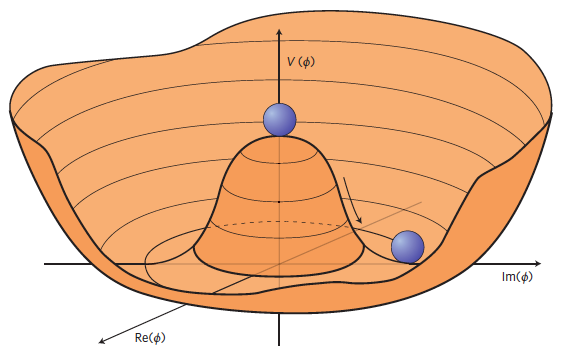
\includegraphics[width=\linewidth,height=\textheight,keepaspectratio]{theory/higgspotential}
        \caption{A two-dimensional representation of the Higgs Potential for a complex Higgs field\cite{higgspotential}.
            Like a ball on a narrow hill, the Higgs field will inevitably roll off to the side into valley below.
            From the Higgs's new perspective at the bottom of this valley,
                the potential no longer appears symmetric,
                leading to the Higgs field acquiring a mass term.
        }
        \label{fig:higgs_potential}
    \end{figure}

    Now for the complications.
    The added symmetries require that the derivative be changed to a covariant derivative 
        $D_{\mu} = \partial_{\mu} - \frac{ig}{2} \wField^a_{\mu} \sigma^a - \frac{ig'}{2} B_{\mu}$.
    Here, $\wField^a_\mu$ and $B_\mu$ correspond to the unbroken $SU(2)$ and $U(1)$ gauge fields respectively.
    This produces a Lagrangian:
    \begin{equation} \begin{split}
        \Lag &= \frac{1}{2} |D_{\mu} \vec{\phi}|^2 +
            \mu^2 \vec{\phi}^\dag \vec{\phi} - \lambda \left( \vec{\phi}^\dag\vec{\phi} \right)^2
        \,.
    \end{split} \end{equation}


    Once again, I allow the scalar field to fall into its offset minimum $v$
        (hereafter referred to as the ``Vacuum Expectation Value'' or \textit{vev})
    \begin{equation}
        v \equiv \frac{\mu}{\sqrt{\lambda}} \textrm{ ,  for   }
            \vec{\phi}(x) \to \vec{h}(x) + \vec{v} = 
            \frac{1}{\sqrt{2}}\minimatrix{0\\h(x)} + \frac{1}{\sqrt{2}}\minimatrix{0\\v} = \frac{1}{\sqrt{2}}\minimatrix{0\\h(x)+v}
        \,.
    \end{equation}
    Worth mentioning is that due to the added groups, there are no longer only two minima.
    Instead, there is now a continuum of equal-valued minima centered on a spherical ``valley'' a distance $v$ from $\phi=0$.
    Substituting into the Lagrangian now produces a more complex expression:
    \begin{equation} \begin{split}
        \label{eq:fullHiggs}
        \Lag & = \frac{1}{2} \left|D_{\mu} \frac{1}{\sqrt{2}}\minimatrix{0\\h(x)+v}\right|^2
            + \mu^2 \left|\frac{1}{\sqrt{2}}\minimatrix{0\\h(x)+v}\right|^2
            - \lambda \left|\frac{1}{\sqrt{2}}\minimatrix{0\\h(x)+v}\right|^4 \\
         & = \Lag_h + \Lag_v
        \,.
    \end{split} \end{equation}
    where $\Lag_h$ takes a form similar to Eqn. \ref{eq:basic_higgs}, incorporating both the $h$ and $h$/$v$ cross terms.
    Meanwhile, $\Lag_v$ refers only to the terms arising from $D_{\mu}$ acting on the vev:
    \begin{equation}
        \label{eq:lagv}
        \Lag_v = \frac{1}{2} (D_{\mu} \vec{v})^2
        \,.
    \end{equation}
    The expansion of this term specifically will lead to the breakdown of Electro-Weak Symmetry,
        and the $W$ and $Z$ bosons acquiring mass.

    %Get covariant derivative, evaluate at vev, pull out W,Z, and photon fields, and their masses (pg 722);
    Expanding only $D_{\mu} \vec{v}$ initially, the $\partial_{\mu}$ immediately vanishes ($v$ is a constant), yielding 
    \begin{equation} \begin{split}
        D^{\mu} v  = \big( \partial^{\mu} & - \frac{ig}{2} \wField^a_{\mu} \sigma^a - \frac{ig'}{2} B_{\mu} \big) \frac{1}{\sqrt{2}}\minimatrix{0\\v} \\
        = \big( & - \frac{ig}{2} \wField^a_{\mu} \sigma^a - \frac{ig'}{2} B_{\mu} \big) \frac{1}{\sqrt{2}}\minimatrix{0\\v} \\
        = - \frac{i}{2} \big( & g \wField^a_{\mu} \sigma^a + g' B_{\mu} \big) \frac{1}{\sqrt{2}}\minimatrix{0\\1} v
        \,.
    \end{split} \end{equation}

    It is useful here to fully expand the $U(1) \times SU(2)$ fields into their matrix components and add them explicitly,
        as doing so reveals the origin of the photon and W and Z bosons.
    \begin{equation} \begin{split}
        g \wField^a_{\mu} \sigma^a + g' B_{\mu} & =
            g \wField^1_{\mu} \sigma^1
            + g \wField^2_{\mu} \sigma^2
            + g \wField^3_{\mu} \sigma^3
            + g' B_{\mu} I \\
        & = \begin{pmatrix}
            0 & g\wField^1_{\mu} \\ g\wField^1_{\mu} & 0 \end{pmatrix}
            + \begin{pmatrix} 0 & -ig\wField^2_{\mu} \\ ig\wField^2_{\mu} & 0 \end{pmatrix}
            + \begin{pmatrix} g\wField^3_{\mu} & 0 \\ 0 & -g\wField^3_{\mu} \end{pmatrix}
            + \begin{pmatrix} g'B_{\mu} & 0 \\ 0 & g'B_{\mu}
        \end{pmatrix} \\
        & = \begin{pmatrix} 
            g\wField^3_{\mu} + g'B_{\mu} & g\wField^1_{\mu} - ig\wField^2_{\mu} \\
            g\wField^1_{\mu} + ig\wField^2_{\mu} & -g\wField^3_{\mu} + g'B_{\mu}
        \end{pmatrix}
        \,.
    \end{split} \end{equation}

    The four components of this matrix will ultimately be associated with the 
        gauge boson fields of the electromagnetic ($A$) and weak ($W$ \& $Z$) interactions
    \begin{equation} \begin{split}
        \label{eq:electroweak_matrix}
        \begin{pmatrix} 
            g\wField^3_{\mu} + g'B_{\mu} & g\wField^1_{\mu} - ig\wField^2_{\mu} \\
            g\wField^1_{\mu} + ig\wField^2_{\mu} & -g\wField^3_{\mu} + g'B_{\mu}
        \end{pmatrix} =
        \begin{pmatrix} 
            \sqrt{g^2 + g^{\prime 2}}\ A_{\mu} & g \sqrt{2}\ W^+_{\mu} \\
            g \sqrt{2}\ W^-_{\mu} & - \sqrt{g^2 + g^{\prime 2}}\ Z^0_{\mu}
        \end{pmatrix}
        \,,
    \end{split} \end{equation}
    with $A$, $W^+$, $W^-$, and $Z^0$ related to the unbroken $\wField^a$ and $B$ fields by
    \begin{equation} \begin{split}
        A_{\mu} & = \frac{1}{\sqrt{g^2 + g^{\prime 2}}} ( g\wField^3_{\mu} + g'B_{\mu} ) \\
        Z^0_{\mu} & = \frac{1}{\sqrt{g^2 + g^{\prime 2}}} ( g\wField^3_{\mu} - g'B_{\mu} ) \\
        W^{\pm}_{\mu} & = \frac{1}{\sqrt{2}} (\wField^1_{\mu} \mp i\wField^2_{\mu})
        \,.
    \end{split} \end{equation}
    The $\sqrt{g^2 + g^{\prime 2}}$ factor is the result of converting between
        $\tinymatrix{Z^0 \\ A}$ and $\tinymatrix{\wField^3 \\ B}$ by way of a rotation matrix
    \begin{equation} \begin{split}
        \begin{pmatrix} Z^0 \\ A \end{pmatrix} =
        \begin{pmatrix}
            \frac{g}{\sqrt{g^2 + g^{\prime 2}}} & \frac{-g'}{\sqrt{g^2 + g^{\prime 2}}} \\
            \frac{g'}{\sqrt{g^2 + g^{\prime 2}}} & \frac{g}{\sqrt{g^2 + g^{\prime 2}}}
        \end{pmatrix} \begin{pmatrix} \wField^3 \\ B \end{pmatrix} = 
        \begin{pmatrix}
            \cos\theta_w & -\sin\theta_w \\
            \sin\theta_w & \cos\theta_w
        \end{pmatrix} \begin{pmatrix} \wField^3 \\ B \end{pmatrix}
        \,,
    \end{split} \end{equation}
    where $\theta_w \equiv \cot(\frac{g'}{g})$ is known as the \textit{weak mixing angle} (AKA the Weinberg angle).

    Returning finally to Eqn. \ref{eq:lagv}, I now have
    \begin{equation} \begin{split}
        \label{eq:lagv_full}
        \Lag_v & = \frac{1}{2} (D_{\mu}^{ij} v_j)^2 \\
        & = \frac{1}{2}
            \frac{1}{\sqrt{2}} \begin{pmatrix} 0 & v \end{pmatrix}
            \left| -\frac{i}{2}
                \begin{pmatrix} 
                    \sqrt{g^2 + g^{\prime 2}}\ A_{\mu} & g \sqrt{2}\ W^+_{\mu} \\
                    g \sqrt{2}\ W^-_{\mu} & - \sqrt{g^2 + g^{\prime 2}}\ Z^0_{\mu}
                \end{pmatrix}
            \right|^2
            \frac{1}{\sqrt{2}} \begin{pmatrix} 0 \\ v \end{pmatrix} \\
        & = \frac{1}{2} \frac{v^2}{2} \frac{1}{4}
            \begin{pmatrix} 0 & 1 \end{pmatrix}
            \begin{pmatrix} 
                \sqrt{g^2 + g^{\prime 2}}\ A_{\mu} & g \sqrt{2}\ W^+_{\mu} \\
                g \sqrt{2}\ W^-_{\mu} & - \sqrt{g^2 + g^{\prime 2}}\ Z^0_{\mu}
            \end{pmatrix}
            \begin{pmatrix} 
                \sqrt{g^2 + g^{\prime 2}}\ A_{\mu} & g \sqrt{2}\ W^+_{\mu} \\
                g \sqrt{2}\ W^-_{\mu} & - \sqrt{g^2 + g^{\prime 2}}\ Z^0_{\mu}
            \end{pmatrix}
            \begin{pmatrix} 0 \\ 1 \end{pmatrix} \\
        & = \frac{1}{2} \frac{v^2}{2} \frac{1}{4}
            \begin{pmatrix} 
                g \sqrt{2}\ W^-_{\mu} & - \sqrt{g^2 + g^{\prime 2}}\ Z^0_{\mu}
            \end{pmatrix}
            \begin{pmatrix} 
                 g \sqrt{2}\ W^+_{\mu} \\
                 - \sqrt{g^2 + g^{\prime 2}}\ Z^0_{\mu}
            \end{pmatrix} \\
        & = \frac{1}{2} \frac{v^2}{2} \frac{1}{4} 
            \left[ 2 g^2  W^-_{\mu} W^+_{\mu}
            + \left(\sqrt{g^2 + g^{\prime 2}}\right)^2 (Z^0_{\mu})^2 \right] \\
        & = \frac{1}{2} \left[ \left(\frac{vg}{2}\right)^2\  W^-_{\mu} W^+_{\mu}
            + \frac{1}{2} \left(\frac{v}{2}\sqrt{g^2 + g^{\prime 2}}\right)^2\ (Z^0_{\mu})^2 \right] \\
        & = \frac{1}{2} \left[ m_W^2 W^{-\ \mu} W^+_{\mu} + \frac{m_Z^2}{2} (Z^0_{\mu})^2 \right]
        \,.
    \end{split} \end{equation}

    As in Section \ref{sec:higgs_mechanism}, the $W$ and $Z$ fields now have additional mass terms associated with their kinetic energy terms,
        with $m_W = \frac{vg}{2}$ and $m_Z = \left(\frac{v}{2}\sqrt{g^2 + g^{\prime 2}}\right) $.
    The photon field $A_{\mu}$ is notably absent in the final Lagrangian, and thus remains massless.
    A similar procedure can then be followed to allow the Higgs Field to interact with fermions
        (albeit with complications arising from mass-mixing and chirality),
        which will grant mass to the Dirac fields.


    % Fermion time!!
%\subsection{Giving Mass to Fermions}
% Ok this is seriously just the same thing but now we have to split the fermion fields into left and right and up-type and down-type
% and split the higgs into the higgs and conjugate higgs and also insert the complex mass matrix except don't insert it for charged leptons
% because reasons or something. And then poof your charged leptons have mass and your quarks have mass and flavour changing

    %Split fermions between right and left fields, assign LH to SU(2) doublets (T=+-1?), RH to SU(2) singlet (T=0), assign Y too (pg724-725);
    %Sandwitch covariant derivative terms between fermion fields, expand to get field currents (pg 725-726);
    %*Try* to expand masses and fail because of representation incompatibilities (pg 725);
    %Anamoly cancellation thing I'll probably ignore (pg 726);
    %Add higgs interaction psibar phi psi to fermion lagrangian, expand into higgs interaction, convert to fermion mass (pg 734);

%Further work must then be done to couple the higgs boson to fermions and itself
%You need to tie k2v, kl, and kv in to the shape of the higgs potential here
\section{Keystone of the Standard Model: The Higgs Boson} \label{sec:higgs_boson}

    With the critical role of the Higgs Field established, it is now time to return to Eqn. \ref{eq:fullHiggs}
        and investigate $\Lag_h$, the Lagrangian of the Higgs boson itself.
    The terms involved therein provide information not only about the Higgs Field,
        but also provide insight into how the Higgs may be further studied:
    \begin{equation} \begin{split}
        \Lag &= \frac{1}{2} |D_{\mu} \vec{\phi}|^2 +
            \mu^2 \vec{\phi}^\dag \vec{\phi} - \lambda \left( \vec{\phi}^\dag\vec{\phi} \right)^2
        \\&= \Lag_K + \Lag_U \quad ; \quad 
            \Lag_K \equiv \frac{1}{2} |D_{\mu} \vec{\phi}|^2 \quad , \quad
            \Lag_U \equiv \mu^2 \vec{\phi}^\dag \vec{\phi} - \lambda \left( \vec{\phi}^\dag\vec{\phi} \right)^2
        \,.
    \end{split} \end{equation}
    
    To make expansion easier, I will expand the covariant derivative terms ($\Lag_K$) first
        and then add the expanded $\Lag_U$ terms.
    Starting with $\Lag_K$, (and defining $Q_{\mu}$ as the matrix from Eqn. \ref{eq:electroweak_matrix})
    \begin{equation} \begin{split}
        \Lag_K &= \frac{1}{2} |D_{\mu} \vec{\phi}|^2
            \\&= \frac{1}{2} (D^{\mu} \vec{\phi})^\dag (D_{\mu} \vec{\phi})
                = \frac{1}{2} \left[(\partial^{\mu} - \frac{i}{2}Q^{\mu}) \vec{\phi}\right]^\dag
                \left[(\partial_{\mu} - \frac{i}{2}Q^{\mu}) \vec{\phi}\right]
            \\&= \frac{1}{2} \left(\vec{\phi}^\dag \partial^{\mu} + \frac{i}{2} \vec{\phi}^\dag Q^{\mu \dag} \right)
                \left(\partial_{\mu}\vec{\phi} - \frac{i}{2}Q_{\mu}\vec{\phi} \right)
            \\&= \frac{1}{2} \left(
                \vec{\phi}^\dag \partial^{\mu} \partial_{\mu}\vec{\phi}
                - \frac{i}{2} \vec{\phi}^\dag \partial^{\mu} Q_{\mu}\vec{\phi}
                + \frac{i}{2} \vec{\phi}^\dag Q^{\mu \dag} \partial_{\mu}\vec{\phi}
                + \frac{1}{4} \vec{\phi}^\dag Q^{\mu \dag} Q_{\mu}\vec{\phi}
                \right)
            \\&= \frac{1}{2} \left(
                | \partial_{\mu}\vec{\phi} |^2
                + \frac{1}{4} \vec{\phi}^\dag Q^{\mu} Q_{\mu} \vec{\phi}
                \right)
                = \frac{1}{2} | \partial_{\mu}h |^2 + \frac{1}{8} \vec{\phi}^\dag Q^{\mu}Q_{\mu} \vec{\phi}
            \\&= \frac{1}{2} | \partial_{\mu}\vec{\phi} |^2 + \frac{1}{8} 
                    \frac{1}{\sqrt{2}}\minimatrix{0 & h^* + v} Q^{\mu}
                    Q_{\mu} \frac{1}{\sqrt{2}}\minimatrix{0 \\ h + v}
            \\&= \frac{1}{2} | \partial_{\mu}h |^2
                + \frac{1}{2} \frac{1}{8} \frac{v^2}{v^2} \left[ 2 g^2  W^-_{\mu} W^+_{\mu}
                + \left(\sqrt{g^2 + g^{\prime 2}}\right)^2 (Z^0_{\mu})^2 \right] (h+v)^2
        \,.
    \end{split} \end{equation}

    The $(h+v)^2$ term will produce couplings quadratic in $v$ ($\Lag_v$ of Eqn. \ref{eq:lagv_full}), and both linear and quadratic in $h$.
    Replacing the coefficients in front of the $W$ and $Z$ fields with their respective masses
        and expanding these terms out (except the quadratic $v$ term, $\Lag_v$) yields
    \begin{equation} \begin{split}
        \Lag_K &= \frac{1}{2} | \partial_{\mu}h |^2
                + \frac{1}{2v^2} \left[ m_W^2\  W^{-\ \mu} W^+_{\mu}
                + \frac{1}{2} m_Z^2\ (Z^0_{\mu})^2 \right] (h+v)^2 \\
        &= \frac{1}{2} | \partial_{\mu}h |^2
            + \frac{1}{v}\left[ m_W^2 W^{-\ \mu} W^+_{\mu} + \frac{m_Z^2}{2} (Z^0_{\mu})^2 \right] h
            + \frac{1}{2v^2} \left[ m_W^2 W^{-\ \mu} W^+_{\mu} + \frac{m_Z^2}{2} (Z^0_{\mu})^2 \right] h^2
            + \Lag_v % FIXME: I'm missing a factor of 2 here :-/
        \,.
    \end{split} \end{equation}

    Often, $W$ and $Z$ field interactions are considered for the same process,
        and as such are described together simply as vector bosons, $V$:
    \begin{equation} \begin{split}
        \Lag_K = \frac{1}{2} | \partial_{\mu}h |^2 + \Lag_v
            + \frac{1}{v} m_V^2 V^2 h + \frac{1}{2v^2} m_V^2 V^2 h^2
        \,.
    \end{split} \end{equation}

    \noindent Returning to $\Lag_U$ and substituting in for $v$
    \begin{equation} \begin{split}
        \Lag_U &= \mu^2 \vec{\phi}^\dag \vec{\phi} - \lambda \left( \vec{\phi}^\dag\vec{\phi} \right)^2
        \\&= - \mu^2 h^2 -\lambda v h^3 - \frac{1}{4} \lambda h^4
        \\&= - \mu^2 h^2 - \mu \sqrt\lambda h^3 - \frac{1}{4} \lambda h^4
        \,.
    \end{split} \end{equation}
    Identifying the Higgs mass $m_h$ as $\sqrt{2}\mu$,
        and the vev $v$ as $\frac{\mu}{\sqrt{\lambda}} = \frac{m_h}{\sqrt{2 \lambda}}$,
        I can now write the full Lagrangian for the Higgs field\cite{Halzen_book}
    \begin{equation} \begin{split} \label{eq:higgsfull}
        \Lag_h &= \Lag_K + \Lag_U
        \\&= \left[ \frac{1}{2} | \partial_{\mu}h |^2
                + \frac{1}{v} m_V^2 V^2 h + \frac{1}{2v^2} m_V^2 V^2 h^2
            \right]
            + \left[ - \frac{1}{2} m^2_h h^2 - m_h \sqrt{\frac{\lambda}{2}} h^3 - \frac{1}{4} \lambda h^4 \right]
        \\&= \frac{1}{2} \left(\partial^2 - m_h^2 \right) h^2
            + \sqrt{2\lambda} \frac{m_V^2}{m_h} V^2 h + \lambda \frac{m_V^2}{m_h^2} V^2 h^2
            - m_h \sqrt{\frac{\lambda}{2}} h^3 - \frac{1}{4} \lambda h^4
        \\&= \frac{1}{2} \left(\partial^2 - m_h^2 \right) h^2
            + g_{HVV} V^2 h + \frac{g_{HHVV}}{2} V^2 h^2
            + \frac{g_{HHH}}{3!} h^3 + \frac{g_{HHHH}}{4!} h^4 \\
        \,.
    \end{split} \end{equation}
    where the coupling terms are defined as
    \begin{equation} \begin{split} \label{eq:higgscouplings}
        g_{HVV}  \equiv 2\sqrt{2\lambda} \frac{m_V^2}{m_h} ,\;
        g_{HHVV} \equiv 4\lambda \frac{m_V^2}{m_h^2} ,\;
        g_{HHH}  \equiv 3\sqrt{2\lambda} m_h ,\;
        g_{HHHH} \equiv 6 \lambda
    \end{split} \end{equation}
    The first term of this Lagrangian is simply the kinetic energy term for the Higgs.
    The remaining terms correspond, respectively,
        to the Higgs/vector boson interaction $g_{HVV}$,
        Higgs/vector boson four-point interaction $g_{HHVV}$,
        Higgs self-coupling $g_{HHH}$,
        and finally the Higgs four-point self-coupling $g_{HHHH}$.

    In 2012, the Higgs boson was detected with a mass of 125 GeV, solidifying both its existence and crucial role in the Standard Model.
    More to the point, its detection confirmed the existence of the Higgs kinetic energy term in the Lagrangian,
        along with its coupling terms to fermions and vector bosons.
    The various self-interaction terms however, are still on more tenuous grounds.
    If they exist at all, there is no guarantee that these interactions have the coupling strength indicated by Eqn. \ref{eq:higgsfull}.
    In order to account for this uncertainty, the Lagrangian can be rewritten with arbitrary scaling factors for the interaction couplings
    \begin{equation} \begin{split} \label{eq:higgskappas}
        \Lag_h &= \frac{1}{2} \left(\partial^2 - m_h^2 \right) h^2
            + \kv g_{HVV} V^2 h + \kvv \frac{g_{HHVV}}{2} V^2 h^2
            + \kl \frac{g_{HHH}}{3!} h^3 + \kappa_{2\lambda} \frac{g_{HHHH}}{4!} h^4
        \,.
    \end{split} \end{equation}

    The new $\kappa$ terms are ratios of the coupling, as predicted by the Standard Model ($g$), to the true coupling value ($g'$).
    The new $\kappa$ terms are ratios of the true coupling value ($g'$)
        to the coupling as predicted by the Standard Model ($g$).
    For example, $\kappa_V \equiv \frac{g'_{HVV}}{g_{HVV}}$.
    A $\kappa$ value of 1 indicates consistency with the coupling strength predicted by the Standard Model.
    Any value other than 1 would indicate deviation from the Standard Model,
        which would need to be explained with a modification to the (or entirely new) theory.
    As of 2020, $\kv$ has been measured at a value of $1.05 \pm 0.04$,
        based on combined analysis of single Higgs production processes\cite{paper:higgs_combined}.
    The couplings $\kvv$, $\kl$, and $\kappa_{2\lambda}$ however, do not significantly affect the production of single Higgs processes.
    The quartic coupling $\kappa_{2\lambda}$ is outside the scope of this thesis,
        but $\kvv$ and $\kl$ can be measured through their effect on di-Higgs production.
    Constraining the range of these values could yield key insight into the validity of the Standard Model and the nature of the Higgs Potential,
        and will therefore be the target of this thesis.


%How do we test any of this?
%From Lagrangian to Cross-Section:
%    I need to study up on exactly how you go from the lagrangian to the Feynman rules, and from there to a calcualable cross section
\section{From Theory to Experiment: The Feynman Rules and Cross-Sections} \label{sec:feyn_rules}
    
    %Justify why we care about cross sections
    After so much discussion of theory, the obvious question to ask is: how can this be tested?
    The most direct physically observable effects of the equations of the Standard Model are those of \textit{differential cross-sections}.
    Cross-sections will be discussed in more detail in Section \ref{sec:lhc-interaction_region},
        but for now it is sufficient to state that the probability of some physical interaction taking place
        is directly proportional to its differential cross-section.
    Here I will provide a general outline for how the Lagrangian of Eqn. \ref{eq:higgskappas} can be related to a measurable cross-section.

    In quantum mechanics, probabilities are defined as the absolute square of amplitudes of wave functions, $\left|\braket{\psi}\right|^2$.
    The probability of a transition between different states of a wavefunction are similarly represented
        as the absolute square of the original state, $\psi_i$, \textit{in the basis of} the final state $\psi_f$,
        written $ |\Tbraket{\psi_f}{\psi_i}|^2$.
    In Quantum Field Theory, states correspond to which particles are in existence at a given moment.
    Thus, a state of one electron and one anti-electron could be written as $\ket{e \bar{e}}$,
        and the transition of an electron-positron pair into a muon/anti-muon pair could be written
        as $\Tbraket{\mu \bar{\mu}}{e \bar{e}}$.

    The process used in this thesis to probe the Higgs's $\kappa$ values is that of
        Vector Boson Fusion (VBF) to a di-Higgs pair decaying to 4b (\vbfhhproc).
    That is, two incoming quarks, $\ket{q_1 q_2}$, form the initial state of this process.
    These quarks each emit a vector boson (either $W^{\pm}$ or $Z^0$), 
        which will in turn fuse into an intermediate state of two Higgs Bosons.
    After being deflected by the weak boson ejection, the quarks then continue on,
        possibly having been flavor-changed if they emitted a charged $W$.
    Meanwhile, the Higgs bosons have a very short lifetime and will decay almost immediately into one of a number of possible particles.
    The likelihood that the Higgs will decay into a given state is given by that state's \textit{branching ratio}.
    As seen from Table \ref{tab:higgsbranching}, a bottom/anti-bottom quark pair is the most likely decay product of the Higgs,
        hence its use as the final state in this analysis.
    The final state of this process consists of two Higgs and the $b \bar{b}$ pairs.
    However, since the Higgs' coupling to the bottom quark does not probe the couplings of interest in this thesis,
        for this chapter I want to focus only on the intermediate state
        consisting of two Higgs and two deflected quarks,
            $\bra{h_1 h_2 q_3 q_4}$.
    I can then write the transition of this process as $\Tbraket{ h_1 h_2 q_3 q_4}{q_1 q_2}$.
    %It should be noted that while there are other intermediate processes besides VBF
    %    that could produce these same initial and final states, 
    %    but these will not be considered in this analysis.

    \begin{table}[tbh]
\begin{center}
\caption{
    Branching ratio of the Higgs to its most common final states.
    The $b \bar{b}$ final state is dominant with over twice the branching ratio of the subleading decay mode,
        and nearly an order of magnitude higher than the sub-sub-leading decay mode\cite{particlephysicsreview2021}.
}
\label{tab:higgsbranching}
%\footnotesize
\begin{tabular}{|l|l|l|}
    \toprule
    Decay channel & Branching ratio & Rel. uncertainty  \\
    \midrule
    $ H \to b \bar{b}        $    & $5.82 \times 10^{-1} $    & $ +1.2\% \atop -1.3\% $ \\
    $ H \to W^+ W^-          $    & $2.14 \times 10^{-1} $    & $\pm 1.5\%        $   \\
    $ H \to \tau^+ \tau^-    $    & $6.27 \times 10^{-2} $    & $\pm 1.6\%        $   \\
    $ H \to c \bar{c}        $    & $2.89 \times 10^{-2} $    & $ +5.5\% \atop -2.0\% $ \\
    $ H \to ZZ               $    & $2.62 \times 10^{-2} $    & $\pm 1.5\%        $   \\
    $ H \to \gamma \gamma    $    & $2.27 \times 10^{-3} $    & $    2.1\%        $   \\
    $ H \to Z \gamma         $    & $1.53 \times 10^{-3} $    & $\pm 5.8\%        $  \\
    $ H \to \mu^+ \mu^-      $    & $2.18 \times 10^{-4} $    & $\pm 1.7\%        $  \\
    \bottomrule
\end{tabular}
\end{center}
\end{table}


    In principle, this transition process can take a finite period of time.
    In the realm of high energy physics experiments though,
        the interacting particles are moving so fast that the interaction period can be thought of as occurring at a single instant in time.
    Given this context, the initial state occurs in the (comparatively) distant past, $t_i$, and the final state in the equally distant future, $t_f$.
    Since the transition occurs at an instantaneous moment,
        I need to perform a time-translation transformation on both states to place them at the moment of the transition, $t_0$.
    Using the Hamiltonian $H \equiv i\partial_0$ as the time translation operator,
        I can relate the initial state at $t_0$ to its time $\Delta t$ units in the future, $t_i$, by the transformation
    \begin{equation}
        \ket{q_{1} q_{2} (t_i)} = e^{i\Delta tH}\ket{q_{1} q_{2} (t_0)}
        \,.
    \end{equation}
    The same can be done to transform the final state backwards in time
    \begin{equation}
        \bra{h_1 h_2 q_{3} q_{4} (t_f)}
        = \bra{h_1 h_2 q_{3} q_{4} (t_0)} (e^{i(-\Delta t)H})^\dag
        = \bra{h_1 h_2 q_{3} q_{4} (t_0)} e^{i\Delta tH}
        \,.
    \end{equation}
    Putting both of these together yields
    \begin{equation} \begin{split} \label{eq:transition_amplitude}
        \Tbraket{ h_1 h_2 q_{3} q_{4} (t_f)}{q_{1} q_{2} (t_i)}
        &= \TbraketA{ h_1 h_2 q_{3} q_{4} (t_0)}{e^{i\Delta tH} e^{i\Delta tH}}{q_{1} q_{2} (t_0)}
        \\&= \TbraketA{ h_1 h_2 q_{3} q_{4} (t_0)}{e^{2\Delta tH}}{q_{1} q_{2} (t_0)}
        \\&= \TbraketA{ h_1 h_2 q_{3} q_{4} (t_0)}{1 + iT}{q_{1} q_{2} (t_0)}
        \,.
    \end{split} \end{equation}

    In the last step, the exponential operator is expanded as an infinite series of terms,
        in a reversal of the procedure from Section \ref{sec:group_theory}.
    The first of these terms will just be 1, corresponding to the static situation in which no interaction occurs at all.
    The sum of the remaining terms, represented as $iT$, is the part relevant for calculating the interaction probability,
        with the entire transition amplitude referred to as the \textit{invariant amplitude}, $\invAmp$:
    \begin{equation}
        i\invAmp \equiv \TbraketA{ h_1 h_2 q_{3} q_{4} (t_0)}{iT}{q_{1} q_{2} (t_0)}
        \,.
    \end{equation}

    As stated above, the differential cross-section, $\dXsec$,
        of a process is proportional to its probability $\mathcal{P}$,
        which in turn can be related to the invariant amplitude
    \begin{equation} \begin{split}
        \dXsec &\propto \mathcal{P}( q_{1} q_{2} \rightarrow q_{3} q_{4} h_1 h_2 ) 
            = \left| \TbraketA{ h_1 h_2 q_{3} q_{4} (t_0)}{iT}{q_{1} q_{2} (t_0)} \right|^2 
            = |i \invAmp|^2 
        \\\dXsec &= \Gamma(p_1, p_2, ...) |\invAmp|^2
        \,.
    \end{split} \end{equation}

    Where $\Gamma(p_1, p_2, ...)$ is a function of the scattering kinematics,
        e.g.\ the particles' crossing angle, energies, and momenta, etc.
    These kinematics are mostly related to the properties of the setup of the scattering experiment under consideration.
    All dependence on the Standard Model Lagrangian is contained within the $\invAmp$ term,
        and the remainder of this chapter will be devoted to its calculation.
    To do this, I turn to Feynman diagrams.

    Calculation of the transition expectation value of the $iT$ term has historically been a very technical challenge.
    Feynman diagrams are an elegant tool for performing this task more easily and intuitively.
    The general process to using them begins with the following steps:
    \begin{itemize}
        \item Draw the initial and final states of the process in question as dots
        \item Fully connect the initial and final state particles using any \textit{valid} intermediate lines and vertices
        \item Valid connections can be identified through the terms present in the Lagrangian:
        \begin{itemize}
            \item Kinetic energy terms correspond to lines connecting a particle to itself
            \item Interaction terms correspond to interaction vertices, connecting three or more particles at a time
            \item All vertices must ensure conservation of any relevant quantum number
        \end{itemize}
        \item Repeat the above steps in order to draw all possible diagrams
    \end{itemize}

    This final step may seem impossible, given that an infinite number of intermediate particles can be inserted between any two states.
    Recall from the structure of $\invAmp$, that $iT$ is not one term, but in fact an infinite series expansion of the Hamiltonian operator.
    For most situations, each higher order of the terms will contribute less to the overall calculation.
    Eventually, the higher-order terms will contribute so little that they can be safely ignored.
    This property is directly reflected in the Feynman Diagrams, in the form of \textit{loops}.
    Any loop in a diagram indicates that the diagram is a higher order term of the expansion.
    A diagram with no loops -- referred as ``tree-level'' or ``leading order'' (LO) -- is part of the first term of $iT$.
    Diagrams with one loop are part of the second term (next-to-leading order, or NLO),
        two loops the third (next-to-next-to-leading order, or NNLO), and so forth.

    One need only draw as many diagrams as is needed for the level of desired precision.
    As a side note, just as successive loops correspond to higher order terms in $iT$,
        diagrams which are not fully connected correspond to the ``1'' term from the original $1+iT$ in Eqn. \ref{eq:transition_amplitude},
        hence why disconnected diagrams are ignored entirely.

    \begin{figure}
    \centering
    \begin{subfigure}{0.32\textwidth} 
        \resizebox{0.9\textwidth}{!}{
\begin{tikzpicture} \begin{feynman}
    \vertex (kv1) {$\kv$};
    \vertex [below=of kv1] (kv2) {$\kv$};
    \vertex [right=of kv1] (h1) {$h_1$};
    \vertex [right=of kv2] (h2) {$h_2$};
    \vertex [above left=of kv1] (vb1);
    \vertex [below left=of kv2] (vb2);
    \vertex [left=of vb1] (q1) {$q_{1}$};
    \vertex [left=of vb2] (q2) {$q_{2}$};

    \vertex [above=of h1] (q3) {$q_{3}$};
    \vertex [below=of h2] (q4) {$q_{4}$};

    \diagram* {
        (q1) -- (vb1) -- (q3),
        (q2) -- (vb2) -- (q4), 
        (vb1) -- [boson] (kv1) -- [boson] (kv2)-- [boson] (vb2),
        (h1) -- [scalar] (kv1),
        (h2) -- [scalar] (kv2),
    };
\end{feynman} \end{tikzpicture}
}
 
        \caption{$M_t$}
        \label{fig:tree_level_vbfhh:kv}
    \end{subfigure}
    \begin{subfigure}{0.32\textwidth}
        \begin{tikzpicture} \begin{feynman}
    \vertex (kv) {$\kv$};
    \vertex [right=of kv] (kl) {$\kl$};
    \vertex [above right=of kl] (h1) {$h_1$};
    \vertex [below right=of kl] (h2) {$h_2$};
    \vertex [above left=of kv] (vb1);
    \vertex [below left=of kv] (vb2);
    \vertex [left=of vb1] (q1i) {$q_{i1}$};
    \vertex [left=of vb2] (q2i) {$q_{i2}$};

    \vertex [above=of h1] (q1f) {$q_{f1}$};
    \vertex [below=of h2] (q2f) {$q_{f2}$};

    \diagram* {
        (q1i) -- (vb1) -- (q1f),
        (q2i) -- (vb2) -- (q2f), 
        (vb1) -- [boson] (kv) -- [boson] (vb2),
        (kv) -- [scalar] (kl),
        (h1) -- [scalar] (kl) -- [scalar] (h2),
    };
\end{feynman} \end{tikzpicture}
 
        \caption{$M_s$}
        \label{fig:tree_level_vbfhh:kl}
    \end{subfigure}
    \begin{subfigure}{0.32\textwidth}
        \resizebox{0.8\textwidth}{!}{
\begin{tikzpicture} \begin{feynman}
    \vertex (k2v) {$\kvv$};
    \vertex [above right=of k2v] (h1) {$h_1$};
    \vertex [below right=of k2v] (h2) {$h_2$};
    \vertex [above left=of k2v] (vb1);
    \vertex [below left=of k2v] (vb2);
    \vertex [left=of vb1] (q1i) {$q_{i1}$};
    \vertex [left=of vb2] (q2i) {$q_{i2}$};

    \vertex [above=of h1] (q1f) {$q_{f1}$};
    \vertex [below=of h2] (q2f) {$q_{f2}$};

    \diagram* {
        (q1i) -- (vb1) -- (q1f),
        (q2i) -- (vb2) -- (q2f), 
        (vb1) -- [boson] (k2v) -- [boson] (vb2),
        (h1) -- [scalar] (k2v) -- [scalar] (h2),
    };
\end{feynman} \end{tikzpicture}
}
 
        \caption{$M_x$}
        \label{fig:tree_level_vbfhh:k2v}
    \end{subfigure}
    \caption{Tree-level diagrams of the \hhproc process.}
    \end{figure}

    Once all possible diagrams have been drawn to the order desired, each diagram has a value assigned to it.
    ``Feynman Rules'' are the rules governing how these values are assigned.
    The rules are derived based on the structure of the Lagrangian and are rather extensive;
        hence, they will not be listed here.
    After the values have been determined, the invariant amplitude is trivially calculated as the sum of the values of all drawn diagrams.
    The \hhproc process studied here is primarily done at tree-level
        (Fig. \ref{fig:tree_level_vbfhh:kv}-\ref{fig:tree_level_vbfhh:k2v}),
        but N\textsuperscript{3}LO calculations are also used to some degree.

    Finally, the differential cross-section can be calculated as the absolute square of the sum of the Feynman Diagrams.
    There is one critical (to this analysis) detail of the Feynman rules I will mention,
        which is that each diagram's value $M$ is proportional to the \textit{product of the coefficients}
        associated with each interaction vertex in the diagram.
    Take for example Fig. \ref{fig:tree_level_vbfhh:kv}, which contains four total vertices;
        two corresponding to the Higgs-Vector Boson interaction (whose coefficient based on Eqn. \ref{eq:higgskappas} is $\kv q_V$),
        and two corresponding to the quark-Vector Boson interaction (whose coefficient is $c_{qV}$).
    As per the Feynman rules, this means that $M_t$ is proportional to $\kv q_V \kv q_V c_{qV} c_{qV}$.
    The quantities I am interested in are of course the $\kappa$ values,
        so I can pull these values out in front of the invariant amplitude as $M_t \rightarrow \kv^2 M_t$.
    At tree-level, I can then write out the absolute square of the invariant amplitude as
    \begin{equation} \begin{split} \label{eq:tree_level_invamp}
        |\invAmp|^2 &= |  \kv^2 M_t + \kv \kl M_s + \kvv M_x |^2
        \\&= \kv^2 \kl^2 M_s^2 + \kv^4 M_t^2 + \kvv^2 M_x^2 
            \\&\qquad + \kv^3 \kl (M_s^* M_t + M_t^* M_s) 
            \\&\qquad + \kv \kl \kvv (M_s^* M_x + M_x^* M_s ) 
            \\&\qquad + \kv^2 \kvv (M_t^* M_x + M_x^* M_t )
        \\\dXsec \propto |\invAmp|^2 &= \kv^2 \kl^2 a_1 + \kv^4 a_2 + \kvv^2 a_3 + \kv^3 \kl a_4 + \kv \kl \kvv a_5 + \kv^2 \kvv a_6
        \,.
    \end{split} \end{equation}

    As noted earlier, the precise value of this cross-section will vary depending on the kinematics of the incoming particles,
        most notably their center of mass (CoM) energy.
    But for this process to occur at all, the CoM energy must be at least the combined mass of the two Higgs Bosons (250 GeV).
    Only a handful of facilities in the world are capable of producing energies at this scale,
        and to produce di-Higgs processes with any appreciable abundance,
        even higher energies are required.
    For measuring the Higgs self-couplings, there is only one machine on the planet that will suffice.

